% Modified Template by Jonathan Doucette and Kevin Multani
% Original Template by Jonathan Ward

% Modified Template by Jonathan Doucette and Kevin Multani, original by: Jonathan Ward

\documentclass[12pt]{article} 
\usepackage[english]{babel}
\usepackage[utf8]{inputenc}
\usepackage{amsmath} % AMS Math Package
\usepackage{amsthm} % Theorem Formatting
\usepackage{amssymb} % Math symbols such as \mathbb
\usepackage{graphicx} % Allows for eps images
\usepackage{multicol} % Allows for multiple columns
\usepackage[dvips,letterpaper,margin=1in,bottom=1in]{geometry}
\usepackage{hyperref}
\usepackage{parskip} % Removes indentation from paragraphs
\usepackage{xcolor,xspace,soul} % Colour, spacing, and highlighting
\usepackage{mathrsfs}
\usepackage{bm} % For bold math symbols
\usepackage{amscd}
\usepackage[all,cmtip]{xy}
%\usepackage{bbm}
\usepackage{titling}
\usepackage{listing} % for code snippets
%\usepackage{minted} % for code snippets
\usepackage{enumerate}
\usepackage{fancyhdr}
\usepackage[]{physics}
\usepackage[makeroom]{cancel}
\usepackage{pdfpages}
\usepackage[]{mcode}
\usepackage[title]{appendix}

% ***********************************************************
% ********************** BEGIN TITLE PAGE *******************
% ***********************************************************
\newcommand*{\titleGM}{\begingroup % Create the command for including the title page in the document
\hbox{ % Horizontal box
\hspace*{0.2\textwidth} % Whitespace to the left of the title page
\rule{1pt}{\textheight} % Vertical line
\hspace*{0.05\textwidth} % Whitespace between the vertical line and title page text
\parbox[b]{0.75\textwidth}{ % Paragraph box which restricts text to less than the width of the page

{\noindent\Huge\bfseries MATH 521}\\[2\baselineskip] % Title
{\large \textit{Assignment 4}}\\[4\baselineskip]
%{\large \textsc{ Jonathan Doucette }} % Author name

\vspace{0.5\textheight} % Whitespace between the title block and the publisher
{\noindent \today }\\[\baselineskip]
%{\noindent Student Number: 35298124 }\\[\baselineskip] 
%{\noindent \footnotesize All problems below are \textit{Copyright \copyright \space 2018 Timm Treskatis. All Rights Reserved.} }\\[\baselineskip]
} % end parbox
} % end hbox
\endgroup}

 % Sets margins and page size
\pagestyle{fancy} 

%\lhead{Jonathan Doucette}
\rhead{\today}
\rfoot{Page \thepage}
\cfoot{}

\makeatletter % Need for anything that contains an @ command 
\renewcommand{\maketitle} % Redefine maketitle to conserve space
{ \begingroup \vskip 10pt \begin{center} \Huge {\bf \@title}
\vskip 10pt \large \@author \hskip 20pt \@date \end{center}
  \vskip 10pt \endgroup \setcounter{footnote}{0} }
\makeatother % End of region containing @ commands

% ***********************************************************
% ********************** END TITLE PAGE *********************
% ***********************************************************

% ***********************************************************
% ********************** BEGIN NEW COMMANDS *****************
% ***********************************************************

\renewcommand{\labelenumi}{(\alph{enumi})} % Use letters for enumerate
\let\vaccent=\v % rename builtin command \v{} to \vaccent{}

%% MISC
\newcommand{\ab}[1]{\left| #1 \right|} % for absolute value
\newcommand{\avg}[1]{\left< #1 \right>} % for average
\let\underdot=\d % rename builtin command \d{} to \underdot{}
\let\baraccent=\= % rename builtin command \= to \baraccent
\renewcommand{\=}[1]{\stackrel{#1}{=}} % for putting numbers above =
\providecommand{\fr}{\frac}
\providecommand{\RR}{\mathbb{R}}
\providecommand{\CC}{\mathbb{C}}
\providecommand{\NN}{\mathbb{N}}
\providecommand{\e}{\epsilon}
\DeclareMathOperator{\di}{d\!}
\newcommand*\ieval[3]{\left.#1\right\rvert_{#2}^{#3}}

%% Vectors
\renewcommand{\v}[1]{\ensuremath{\mathbf{#1}}} 
\newcommand{\gv}[1]{\ensuremath{\mbox{\boldmath$ #1 $}}} % for vectors of Greek letters
\newcommand{\uv}[1]{\ensuremath{\mathbf{\hat{#1}}}} % for unit vector
\providecommand{\wave}[1]{\v{\tilde{#1}}}

%% DERIVATIVES
\renewcommand{\d}[2]{\frac{d #1}{d #2}} % for derivatives
\newcommand{\dubd}[2]{\frac{d^2 #1}{d #2^2}} % for double derivatives
\newcommand{\pd}[2]{\frac{\partial #1}{\partial #2}} % for partial derivatives
\newcommand{\pdd}[2]{\frac{\partial^2 #1}{\partial #2^2}} % for double partial derivatives

%% Operators
\newcommand{\Gradient}{\ensuremath{\mbox{\boldmath$\nabla$}}} % gradient

%% Text
\newcommand{\mathcolorbox}[2]{\colorbox{#1}{$\displaystyle #2$}}
\newcommand{\hlfancy}[3]{\textcolor{#1}{\sethlcolor{#2}\hl{#3}}}
\newcommand{\TODO}[1]{\hlfancy{red}{yellow}{\textbf{TODO: #1}}}

%% Code
%\newcommand{\code}[1]{\mintinline{C}{#1}}
%\newcommand{\code}[1]{\texttt{#1}}
\newcommand{\code}[1]{\lstinline[columns=fixed]{#1}}
\newcommand{\includecode}[1]{\lstinputlisting{#1}}

% ***********************************************************
% ********************** END NEW COMMANDS *******************
% ***********************************************************

% ***********************************************************
% ********************** BEGIN NEW ENVS *********************
% ***********************************************************

% Theorem
\newenvironment{theorem}[2][Theorem]{\begin{trivlist}
\item[\hskip \labelsep {\bfseries #1}\hskip \labelsep {\bfseries #2.}]}{\end{trivlist}}
% Lemma
\newenvironment{lemma}[2][Lemma]{\begin{trivlist}
\item[\hskip \labelsep {\bfseries #1}\hskip \labelsep {\bfseries #2.}]}{\end{trivlist}}
% Corollary
\newenvironment{corollary}[2][Corollary]{\begin{trivlist}
\item[\hskip \labelsep {\bfseries #1}\hskip \labelsep {\bfseries #2.}]}{\end{trivlist}}

% Exercise
\newenvironment{exercise}[2][Exercise]{\begin{trivlist}
\item[\hskip \labelsep {\bfseries #1}\hskip \labelsep {\bfseries #2.}]}{\end{trivlist}}
% Problem
\newenvironment{problem}[2][Problem]{\begin{trivlist}
\item[\hskip \labelsep {\bfseries #1}\hskip \labelsep {\bfseries #2.}]}{\end{trivlist}}
% Question
\newenvironment{question}[2][Question]{\begin{trivlist}
\item[\hskip \labelsep {\bfseries #1}\hskip \labelsep {\bfseries #2.}]}{\end{trivlist}}
% Solution
\newenvironment{solution}{\begin{proof}[Solution]}{\end{proof}}

% Afterword
\newenvironment{afterword}[2][Appendix]{\begin{trivlist}
\item[\hskip \labelsep {\bfseries #1}\hskip \labelsep {\bfseries #2}]}{\end{trivlist}}

% ***********************************************************
% ********************** END NEW ENVS ***********************
% ***********************************************************

% ***********************************************************
% ********************** END TITLEPAGE **********************
% ***********************************************************

\begin{document}

\begin{titlingpage}
	\titleGM
\end{titlingpage}
\clearpage
\setcounter{page}{1}

%%%%%%%%%%%%%%%%%%%%%%%%%
% ----- PROBLEM 1 ----- %
%%%%%%%%%%%%%%%%%%%%%%%%%
\begin{problem}{1}
Given three points $a,b,c \in \RR^2$ that are not collinear (not all on one line) and that are sorted in anticlockwise order, we define
%
\begin{align*}
T &= \Delta (a,b,c) \\
P &= P_2(T) \\
L &= \left\{ \vphantom{\pd{p}{n}\left(\frac{a+b}{2}\right)} \right.
p \mapsto p(a),
p \mapsto p(b),
p \mapsto p(c), \\
&\qquad\quad
p \mapsto \pd{p}{n}\left(\frac{a+b}{2}\right),
p \mapsto \pd{p}{n}\left(\frac{b+c}{2}\right),
\left. p \mapsto \pd{p}{n}\left(\frac{c+a}{2}\right) \right\}
\subset P*
\end{align*}

\begin{center}
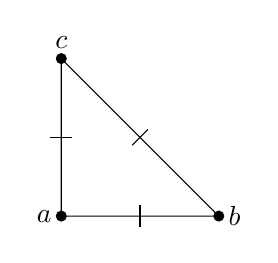
\begin{tikzpicture}
\draw (0,0) node[anchor=east]{$a$}
  -- (2,0) node[anchor=west]{$b$}
  -- (0,2) node[anchor=south]{$c$}
  -- cycle;
\fill (0,0) circle[radius=2pt];
\fill (2,0) circle[radius=2pt];
\fill (0,2) circle[radius=2pt];
\draw (1,-0.14) -- (1,0.14);
\draw (-0.14,1) -- (0.14,1);
\draw (1-0.1,1-0.1) -- (1+0.1,1+0.1);
\end{tikzpicture}
\end{center}

% ----- Problem 1(a) ----- %
\begin{itemize}
	\item[(a)]  Show that prescribed data for
	$$p \mapsto p(a),
	p \mapsto p(b),
	p \mapsto p(c),
	p \mapsto \pd{p}{n}\left(\frac{a+b}{2}\right),
	p \mapsto \pd{p}{n}\left(\frac{b+c}{2}\right),
	p \mapsto \pd{p}{n}\left(\frac{c+a}{2}\right)$$
	uniquely determines any $p \in P$. You don't have to show that such a $p$ always exists.

\end{itemize}

% ----- Problem 1(a): Solution ----- %
\begin{solution}
A general second order polynomial in two-dimensions takes the form
\begin{equation}\label{QuadInterpPoly}
p(x) = A_1 x_1^2 + A_2 x_1x_2 + A_3 x_2^2 + A_4 x_1 + A_5 x_2 + A_6,
\end{equation}
where $x = (x_1,x_2) \in \RR^2$, as the space $P_2(T)$ is given by
$$P_2(T) = \spann \{ 1,\, x_1,\, x_2,\, x_1 x_2,\, x_1^2,\, x_2^2 \}.$$
Since $p$ has 6 unknown coefficients, 6 conditions on $p$ are required in order to determine the coefficients $A_i$ (assuming non-degeneracy of the prescribed conditions).
The prescribed conditions are those in $L$, which we will show produces a unique polynomial $p$.

Suppose we take $L$ to be the special case $L_0$ of all-zero conditions, where
\begin{equation}\label{L0conds}
p_0(a) = p_0(b) = p_0(c) =
\pd{p_0}{n}\left(\frac{a+b}{2}\right) =
\pd{p_0}{n}\left(\frac{b+c}{2}\right) = 
\pd{p_0}{n}\left(\frac{c+a}{2}\right) = 0.
\end{equation}
Then, if we can show that the polynomial $p_0 \in P_2(T)$ which satisfies $L_0$ is exactly the zero solution $p_0 \equiv 0$, we will have shown uniqueness for the general case of $p$ satisfying $L$ due to the fact that we have linear degrees of freedom $A_i$.

We start by considering the normal derivative conditions.
Since $p_0$ is second order in $x_1$ and $x_2$, it follows that the normal derivative $\pd{p_0}{n} = \nabla{p_0} \cdot n$ is a linear function of $x_1$ and $x_2$, as
\begin{equation}\label{p0grad}
\nabla{p_0} = \begin{bmatrix}
2A_1 x_1 + A_2 x_2 + A_4 \\ 
A_2 x_1 + 2 A_3 x_2 + A_5
\end{bmatrix}
\end{equation}

is a linear function in $x_1$ and $x_2$, and $n$ is a constant vector.

Let us consider the tangential component of the gradient. Denote $t$ the unit vector pointing from $a$ to $b$. Then, by the fundamental theorem of vector calculus,
\begin{align*}
\int_{a\rightarrow b} \nabla{p_0} \cdot d\vec{s} &= \int_{a\rightarrow b} \pd{p_0}{t} ds \\
&= p_0(b) - p_0(a) \\ 
&= 0.
\end{align*}
Thus, the \textit{average} value of the tangential component of the gradient, $\pd{p_0}{t}$, must be zero along the line segment.
Now, since $\pd{p_0}{t}$ is linear, this means that $\pd{p_0}{t}$ must be zero at the midpoint:
$$ \pd{p_0}{t}\left(\frac{a+b}{2}\right) = 0.$$
We are given that $\pd{p_0}{n}$ is zero at the midpoint as well, and so the full gradient $\nabla{p_0}$ is zero at the midpoint.
This argument holds for all three sides, and so we have that 
$$\nabla{p_0} = 0$$
at all three midpoints.
Note that $\nabla{p_0} = 0$ implies all directional derivatives are zero at that point, including partial derivatives $\pd{p_0}{x}$ and $\pd{p_0}{y}$.

The gradient $\nabla{p_0}$ given by equation \ref{p0grad} shows that $\pd{p_0}{x}$ and $\pd{p_0}{y}$ are given by plane equations (linear equations in $x_1$ and $x_2$).
Since planes are defined by their values at three points, and we have that $\pd{p_0}{x} = \pd{p_0}{y} = 0$ at all three edge midpoints, it must be that $\pd{p_0}{x} \equiv 0$ and $\pd{p_0}{y} \equiv 0$ on all of $T$, and thus $\nabla{p_0} \equiv 0$ on all of $T$.

Finally, $\nabla{p_0} \equiv 0$ implies that $p_0$ must be constant on $T$, and since $p_0$ takes the value $0$ at all three corners, it must be that $p_0 \equiv 0$ identically.

Uniqueness of $p$ for generic data $L$ follows, as previously stated.

\end{solution}
\pagebreak

% ----- Problem 1(b) ----- %
\begin{itemize}
	\item[(b)] Now let $\Omega^h$ be a domain with a regular triangulation $T^h$ such that
	$$\bar{\Omega}^h = \bigcup_{T\in T^h} T.$$
	Is the space
	\begin{gather*}
	V^h = \left\{ \vphantom{\pd{v^h}{n}}
	v^h \colon \bar{\Omega}^h \rightarrow \RR \:\middle|\:
	v^h\!\mid_T\, \in P_2(T), v^h\,\text{is continuous in all vertices},
	\right. \\ \left.
	\pd{v^h}{n}\,\text{is continuous in all edge midpoints}
	\right\}
	\end{gather*}	 
	$H^1$-conforming, i.e. is $V^h \subset H^1(\Omega^h)$?
	\textit{Hint:} Check if there may be any jumps of $v^h$ across triangle edges.
\end{itemize}

% ----- Problem 1(b): Solution ----- %
\begin{solution}
We start by considering a generic triangle edge.
We use the notation that this edge connects points $a$ and $b$ in the plane which belong to adjacent triangles $T_1$ and $T_2$, and we denote $v^h_1 \in P_2(T_1)$ and $v^h_2 \in P_2(T_2)$ the quadratic interpolating polynomials on the respective triangles, each taking the form \ref{QuadInterpPoly}.

%This edge lies on a line, denoted $\gamma$, given by the linear equation
%\begin{equation}\label{gamma}
%B_1 x_1 + B_2 x_2 + B_3 = 0
%\end{equation}
%where the coefficients $B_i$ depend on $a$ and $b$.
%Now, consider the values that the polynomial $v^h_1$ can take on $\gamma$; thinking of $\gamma$ as a constraint on $v^h_1$, we see that (e.g. by solving for $x_1$ or $x_2$ in \ref{gamma} and plugging the result into $v^h_1$) the bivariate quadratic polynomial $p$ reduces to a univariate quadratic polynomial on the line $\gamma$, which we denote
%$$ v^h_1(t) = C_1 t^2 + C_2 t + C_3. $$
%By the same argument, $v^h_2$ takes a similar form.

Now, we know that $v^h_1$ and $v^h_2$ match at the end points, so the difference $e^h = v^h_1 - v^h_2$ is zero at $a$ and $b$.
Additionally, since $\pd{v^h_1}{n} = \pd{v^h_2}{n}$ at the midpoint, $\pd{e^h}{n} = 0$ at the midpoint. Using the same argument as in Problem 1(a), due to the linearity of the gradient and the fact that $e^h$ is zero at both endpoints, $\pd{e^h}{t} = 0$ at the midpoint and so $\nabla{e^h} = 0$ at the midpoint.

However, we have no guarantees for the function values away from the edges; there are too many degrees of freedom.
Consider the following counterexample:
\begin{align*}
v^h_1 &= (x_1^2 - 1) - x_2 + 1 \\
v^h_2 &= 2(x_1^2 - 1) + x_2 + 1
\end{align*}
where $T_1$ has vertices $a_1=(-1,0)$, $b_1=(1,0)$, and $c_1=(0,1)$, and $T_2$ has vertices $a_2=(-1,0)$, $b_2=(0,-1)$, and $c_2=(1,0)$.
$T_1$ and $T_2$ are the top and bottom half, respectively, of the ``diamond'' with vertices at $(\pm 1,0)$ and $(0,\pm 1)$, and are connected by their shared edge $e$ which lies on the line $x_2 = 0$.

Now, it is clear that on $v^h_1(\pm 1,0) = v^h_2(\pm 1,0) = 1$, i.e. they are equal at the endpoints of $e$.
Additionally, since the normal direction to $e$ is $-x_2$ on $T_1$ and $+x_2$ on $T_2$, we have that $\pd{v^h_1}{n}(0,0) = \pd{v^h_2}{n}(0,0) = 1$, i.e. the normal derivatives are continuous at the midpoints.
However, clearly $v^h_1 \neq v^h_2$ anywhere else on $e$ (where $x_2=0$).

In conclusion, \textbf{$V^h$ is not $H^1$-conforming}, due to the fact that jumps of $v^h$ across triangle edges is indeed possible in general.

%is a univariate quadratic polynomial (on $\gamma$) which is zero at both $a$ and $b$, and therefore has only one degree of freedom.

%We can show that $e^h$ is zero at the midpoint $\frac{a+b}{2}$ as well by using the fact that $\pd{v^h_1}{n} = \pd{v^h_2}{n}$ at $\frac{a+b}{2}$.

\end{solution}
\pagebreak

\end{problem} % END PROBLEM 1
\pagebreak

%%%%%%%%%%%%%%%%%%%%%%%%%
% ----- PROBLEM 2 ----- %
%%%%%%%%%%%%%%%%%%%%%%%%%
\begin{problem}{2}
We will now complete our finite-element solver for the linear elasticity problem
\begin{align}\label{LinElast_Strong}
\begin{split}
    -c \Laplacian u + au &= f \quad \text{in } \Omega \\
    u &= g \quad \text{on } \partial \Omega
\end{split}
\end{align}

% ----- Problem 2 ----- %
\begin{itemize}
	\item[(a)] Remove lines 1-10 from \code{discretiseLinearElasticity.m} and uncomment the sections of code that are currently commented out.
	Complete the missing commands, including the subfunction \code{assembleStiffness}. Also inspect the \code{assembleLoad} subfunction.

% ----- Problem 2(a) Solution ----- %
\begin{solution}
The finished function \code{discretiseLinearElasticity.m} and subfunction \\ \code{assembleStiffness} is included in Appendix\ref{discLinElastCode}.
\end{solution}
\pagebreak

	\item[(b)] Write a script \code{hw6.m} which
	\begin{itemize}
		\renewcommand{\labelitemii}{$\bullet$}
	    \item Solves the linear elasticity problem on $\Omega^h$, which you may choose from kiwi.mat, maple.mat, pi.mat, ubc.mat.
	    You may also select your own data for $f(x_1,x_2)$, $g(x_1,x_2)$, $a$ and $c$. \\\\
	    \textit{Hint:} You have to set \code{GammaD = @(x1,x2) true(size(x1))}.
	    For debugging, you might want to use \code{video10.mat} and check the sparsity patterns of the various matrices.
	    \item Calculates the $L^2$, $H^1$, and $B$ energy norms of the solution, where $B$ is the bilinear form corresponding to the elliptic operator.
	    \item Creates undistorted plots of the mesh, the force $f$, and the solution $u^h$.
	\end{itemize}

% ----- Problem 2(b) Solution ----- %
\begin{solution}
The script \code{hw6.m} is included in Appendix~\ref{hw6Code}.

I chose to use the \code{maple.mat} dataset.
The mesh and sparsity patterns of the mass and stiffness matrices are plotted below.
For the forcing function, I used a constant forcing $f\equiv 1$ with fixed Dirichlet boundaries $g \equiv 0$, as it is the most intuitive to tell if the solution looks right or not (should bend more in the flat regions than narrow regions/near edges).

\vspace{0.7cm}
\begin{figure}[ht]
\centering
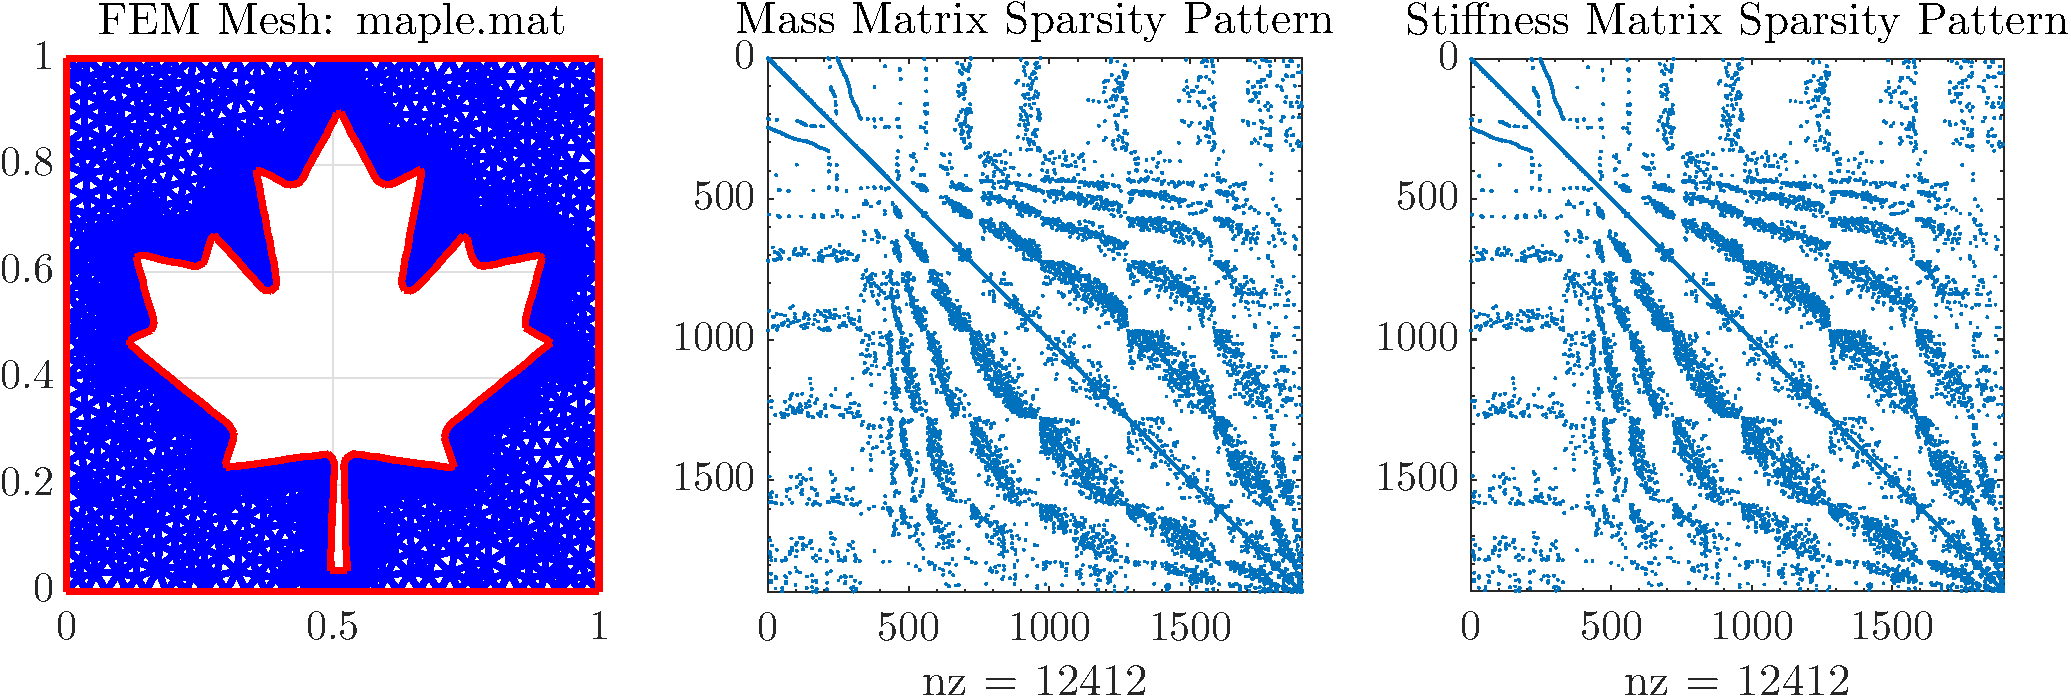
\includegraphics[width=1.0\textwidth]{../maple-mesh}
\caption{Mesh and sparsity patterns of the mass and stiffness matrices for the \code{maple.mat} data set.}\label{maple-mesh}
\end{figure}

\pagebreak
\begin{figure}[ht]
\centering
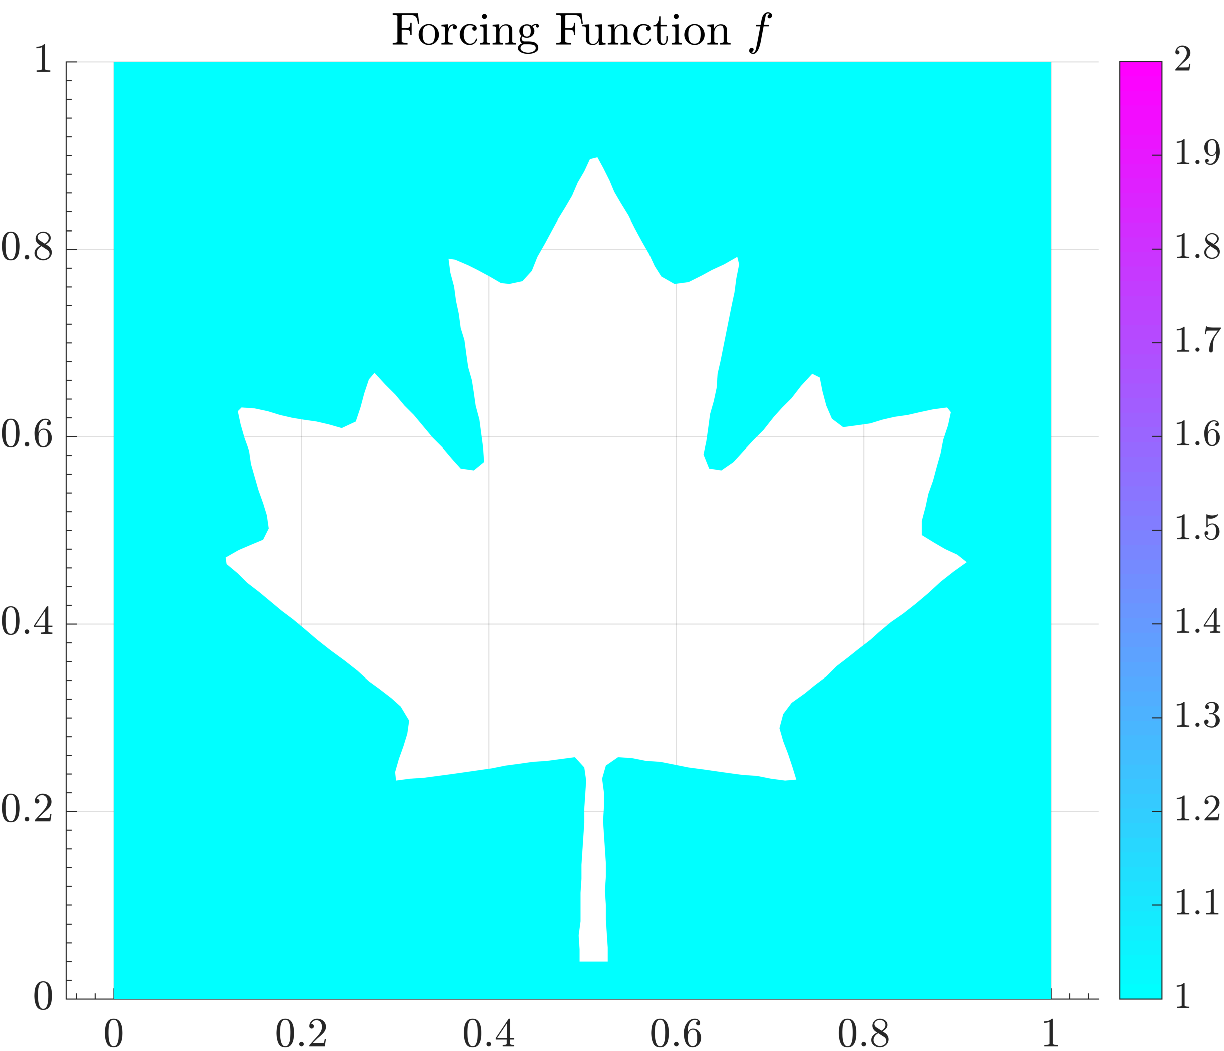
\includegraphics[width=1.0\textwidth]{../maple-const-force}
\caption{Plot of the constant forcing function $f\equiv 1$ on the \code{maple.mat} finite elements mesh.}\label{maple-const-force}
\end{figure}

\pagebreak
\begin{figure}[ht]
\centering
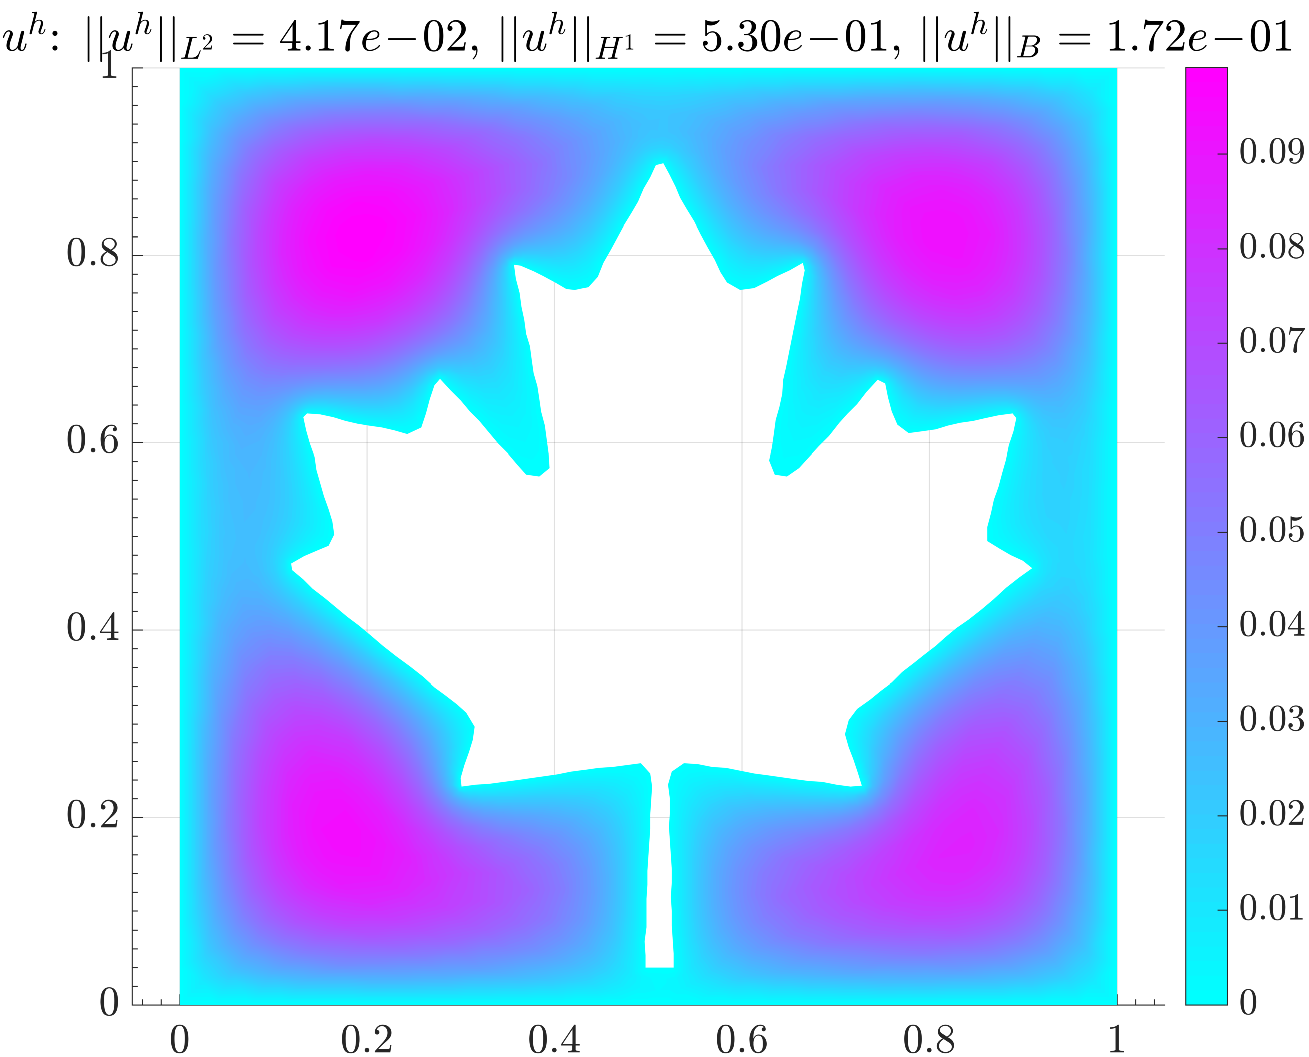
\includegraphics[width=1.0\textwidth]{../maple-soln}
\caption{Plot of the solution function $u^h$ corresponding to the constant forcing function $f\equiv 1$ on the \code{maple.mat} finite elements mesh, with relevant norms computed.}\label{maple-soln}
\end{figure}

\end{solution}
\pagebreak

	\item[(c)] What problem do you solve numerically when you set \code{GammaD = @(x1,x2) false(size(x1))}?
	Analyse the code to infer its weak formulation.
\end{itemize}

% ----- Problem 2: Solution ----- %
\begin{solution} 
Setting \code{GammaD = @(x1,x2) false(size(x1))} would result in no Dirichlet boundary points prescribed with the boundary data $g(x_1,x_2)$, which result in all boundary points being free.

In terms of code, these means that the matrix free projection matrix \code{Pf} would be the identify matrix.
The reduced linear system defined by \code{A} and \code{b} would become the full system and would be equivalent to
\begin{align*}
&\code{A = c*Kbar + a*Mbar;}\\
&\code{b = fbar;}
\end{align*}

The weak form in it's discretized form is therefore given by
\begin{align*}
    \sum_{i=1}^N \bigg(
    c \int_\Omega \nabla \phi_i^h \cdot \nabla \phi_j^h \dx{x} + 
    a \int_\Omega \phi_i^h \phi_j^h \dx{x} 
    \bigg) u_j^h = 
    \int_\Omega f \phi_i^h \dx{x},
\end{align*}
where \textit{all} values $u^h_j$ are free.
The non-discretized form is then given by
\begin{align}\label{LinElast_Weak}
c \int_\Omega \nabla u \cdot \nabla v \dx{x} + 
a \int_\Omega u v \dx{x} = 
\int_\Omega f v \dx{x}.
\end{align}

\end{solution}
\pagebreak

\end{problem} % END PROBLEM 2
\pagebreak


%%%%%%%%%%%%%%%%%%%%%%%
% ----- WRITTEN ----- %
%%%%%%%%%%%%%%%%%%%%%%%
\begin{afterword}[Your Learning Progress]{}
What is the one most important thing that you have learnt in this assignment?
\vspace{0.2cm}

That it is very non-trivial to determine properties of finite elements!
Especially with regards to uniqueness and existence proofs.

\vspace{0.8cm}
Any new discoveries or achievements towards the objectives of your course?
\vspace{0.2cm}

I'm starting to like finite element methods a lot more!
Quite finicky, but worthwhile.

\vspace{0.8cm}
What is the most substantial new insight that you have gained from this course this week? Any \textit{aha moment}?
\vspace{0.2cm}

Only that it is not at all obvious whether or not a finite element will be a valid one or not without doing the analysis.

\end{afterword}

\pagebreak

%%%%%%%%%%%%%%%%%%%%
% ----- CODE ----- %
%%%%%%%%%%%%%%%%%%%%
\begin{appendices}
\lhead{}

\section{}\label{discLinElastCode}
The \code{discretiseLinearElasticity.m} function:
\includecode{../../Library/discretiseLinearElasticity.m}
\pagebreak
\section{}\label{hw6Code}
The \code{hw6.m} script:
\includecode{../hw6.m}

\end{appendices}

\end{document}
